\section{Алгоритм рендеринга черной дыры со сторонней геометрией}
\label{sec:Chapter3} \index{Chapter3}

В реальности источниками искривления пространства-времени являются любые объекты, имеющие массу. Однако на фоне черных дыр большинство из них имеют пренебрежимо малую массу, а значит практически не искривляют пространство. Данная глава посвящена визуализации черной дыры именно с маломассивными объектами.

\subsection{Трассировка лучей в компьютерной графике}

\begin{figure}[h]
    \centering
    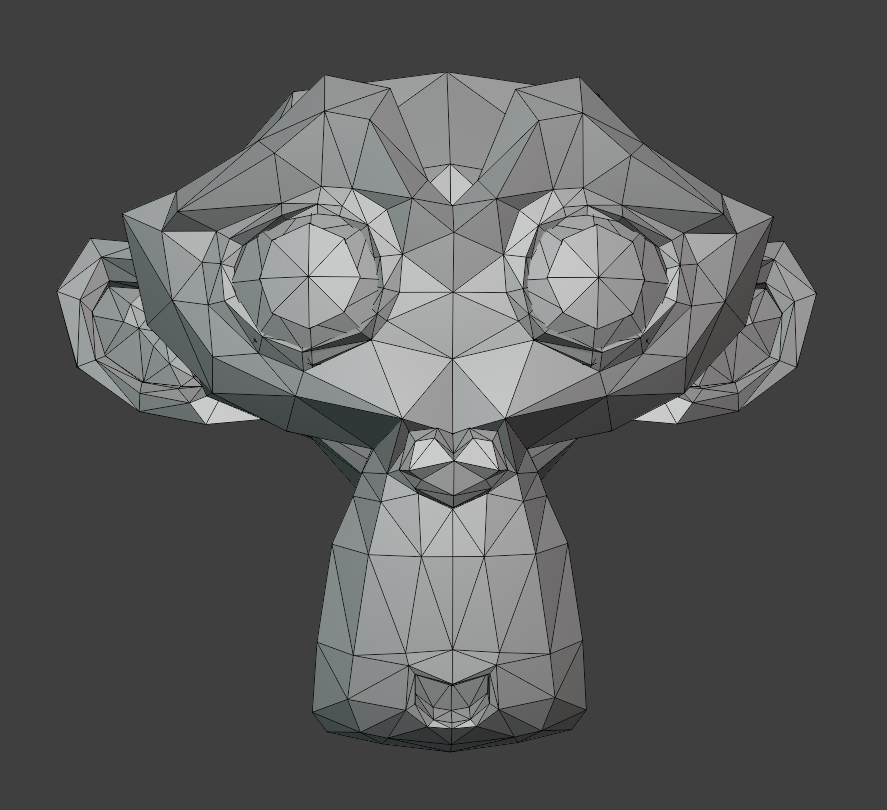
\includegraphics[width=0.7\linewidth]{Monkey}
    \caption{Пример построения головы примата из набора треугольников.}
    \label{fig:monkey}
\end{figure}

Самым популярным способом представления объектов в компьютерной графике является набор треугольников (см. рис. \ref{fig:monkey}), поэтому в дальнейшем предполагается, что объекты состоят из треугольников.

Известно, что объект является видимым, если в глаз (камеру) попадет луч света от этого объекта. Пользуясь законом обратимости света, если луч, выпущенный из нашего глаза (камеры) попадет в объект, то объект можно считать видимым. Таким образом для каждого луча на сцене необходимо делать проверку на пересечение со всеми объектами и если пересечение произошло, то обрабатывать его в зависимости от свойств объекта. В данной работе используется упрощенная модель отрисовки объектов: при пересечении луча с объектом, луч приобретает цвет объекта в точке пересечения.

В неевклидовых пространствах луч света не всегда движется по прямой. Траектория света может быть даже не представима в аналитическом виде. В качестве решения этой проблемы траекторию света можно приблизить ломаной линией и на отрезках, соединяющих известные точки траектории, совершать проверку на пересечение с объектами. Однако эти точки должны быть расположены достаточно близко, чтобы ломаная линия была мало отличима от настоящей траектории движения света. Для каждого искривленного пространства свои критерии на это условие, однако для черной дыры критерий следует из \eqref{eq:diffur} и выглядит так:

\begin{equation}
    \Delta\tan{\alpha} = -r\frac{d^2u}{d\phi^2}\Delta\phi = -r\left( \frac{3}{2}r_s\left(\frac{1}{r}\right)^2 - \frac{1}{r} \right)\Delta\phi \ll 1.
\end{equation}
, то есть изменение угла $\alpha$ (см. рис. \ref{fig:transform_direction} и \ref{fig:angle_overview}) должно быть малым при выбранном малом изменении угла $\phi$, что всегда выполняется.

Таким образом, поиск пересечения траектории света с объектами свелся к поиску пересечения отрезков (из которых состоит приближенная траектория света) с треугольниками (из которых состоит объект). В компьютерной графике такое называется \textit{трассировкой лучей}.

\subsection{Усовершенствованный алгоритм рендеринга черной дыры}
\label{subsec:new_algos}

\begin{figure}[h]
    \centering
    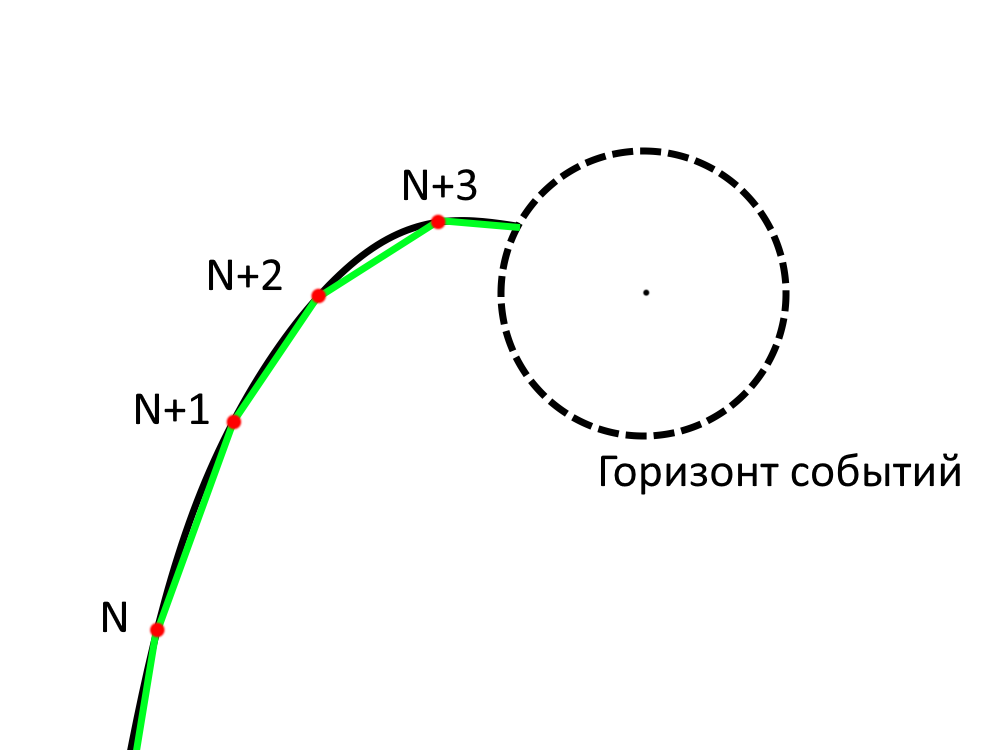
\includegraphics[width=0.7\linewidth]{BlackHole-RayMarchingTracing-Overview}
    \caption{Усовершенствованный алгоритм рендеринга черной дыры. Зеленые отрезки - отрезки, на которых совершается проверка пересечения этого отрезка с объектами сцены.}
    \label{fig:blackhole_raymarchingtracing}
\end{figure}

Используя алгоритмы пересечения луча с треугольниками, можно находить точки их пересечения. Таким образом, пользуясь алгоритмом из раздела \ref{subsec:algos}, можно между каждыми точками итерации совершать проверку на пересечение (см. рис. \ref{fig:blackhole_raymarchingtracing}). Тогда алгоритм рендеринга черной дыры с объектами будет выглядить следующим образом (\textit{курсивом} обозначена новая часть алгоритма):

\begin{enumerate}
    \item Инициализация лучей света (раздел \ref{subsec:ray_init}).
    \item Переход из декартовых координат в полярные координаты плоскости вращения (раздел \ref{subsec:transition_from_decart_to_polar}).
    \item В бесконечном цикле решения дифференциального уравнения методом Рунге-Кутты:
    \begin{enumerate}
        \item Проверка краевых случаев (раздел \ref{subsec:corner_cases}):
        \begin{enumerate}
            \item Проверка на нахождение в горизонте событий (раздел \ref{subsubsec:events_horizon}).
            \item Проверка на уход в бесконечность (раздел \ref{subsubsec:goes_to_infinity}).
        \end{enumerate}
        \item Получение новой точки итерации методом Рунге-Кутты (раздел \ref{subsec:runge-kutte}).
        \item Переход из полярных координат плоскости вращение в декартовы (раздел \ref{subsec:transition_from_polar_to_decart}).
        \item \textit{Проверка на пересечение объектов с отрезком, соединяющим новую и предыдущую точки итерации. Выполнение обработки пересечения при его нахождении.}
        \item Добавление к итоговому цвету цвета аккреционного диска (раздел \ref{subsec:accr_disk}).
    \end{enumerate}
\end{enumerate}

Этот алгоритм представляет из себя комбинацию марширования лучей и трассировки лучей.

\begin{figure}[h]
    \centering
    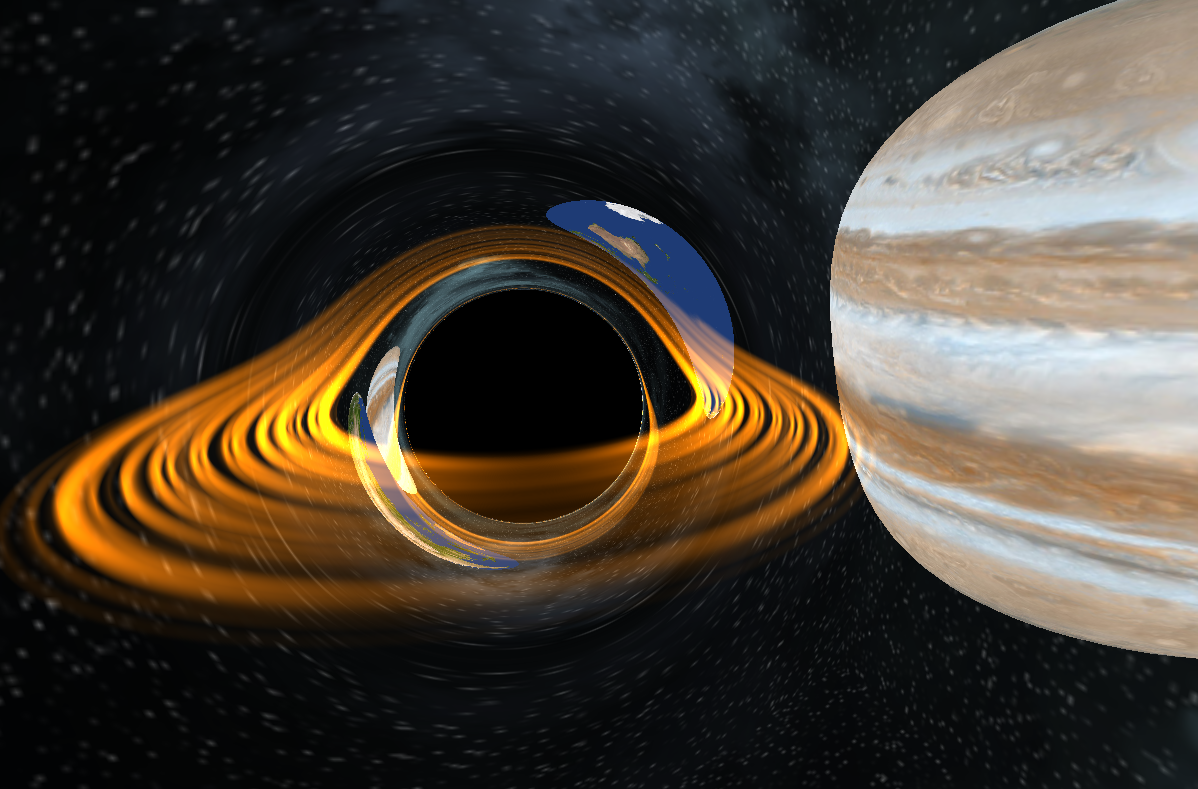
\includegraphics[width=1.0\linewidth]{BlackHole-RayTracing}
    \caption{Визуальный результат усовершенствованного алгоритма рендеринга черной дыры со сторонней геометрией.}
    \label{fig:blackhole_raytracing}
\end{figure}

На рисунке \ref{fig:blackhole_raytracing} представлен итоговый визуальный результат усовершенствованного метода рендеринга черной дыры со сторонней геометрией. Известно, что хоть Юпитер находиться ближе к камере, чем Земля, в более искривленном их изображении слева от черной дыры Земля перекрывает Юпитер, потому что в ходе движения луча с этой стороны от черной дыры луч сперва сталкивается с Землей, а уже потом (если бы луч умел проходить сквозь объекты) с Юпитером.

\newpage